\begin{frame}{Seat Planning with Social Distancing}
  Prerequisite: people in one group should sit together.
  \begin{itemize}  
    \item Group type $\mathcal{M} = \{1, \ldots, M\}$.
    \item Row $\mathcal{N} = \{1, \ldots, N\}$.
    \item The social distancing: $\delta$ seat(s).
    \item $n_i = i + \delta$: the new size of group type $i$ for each $i \in \mathcal{M}$.
    \item The number of seats in row $j$: $L_j^{0}, j \in \mathcal{N}$.
    \item $L_j = L_j^{0} + \delta$: the length of row $j$ for each $j \in \mathcal{N}$.
    \end{itemize}
    
    \begin{figure}[ht]
      \centering
      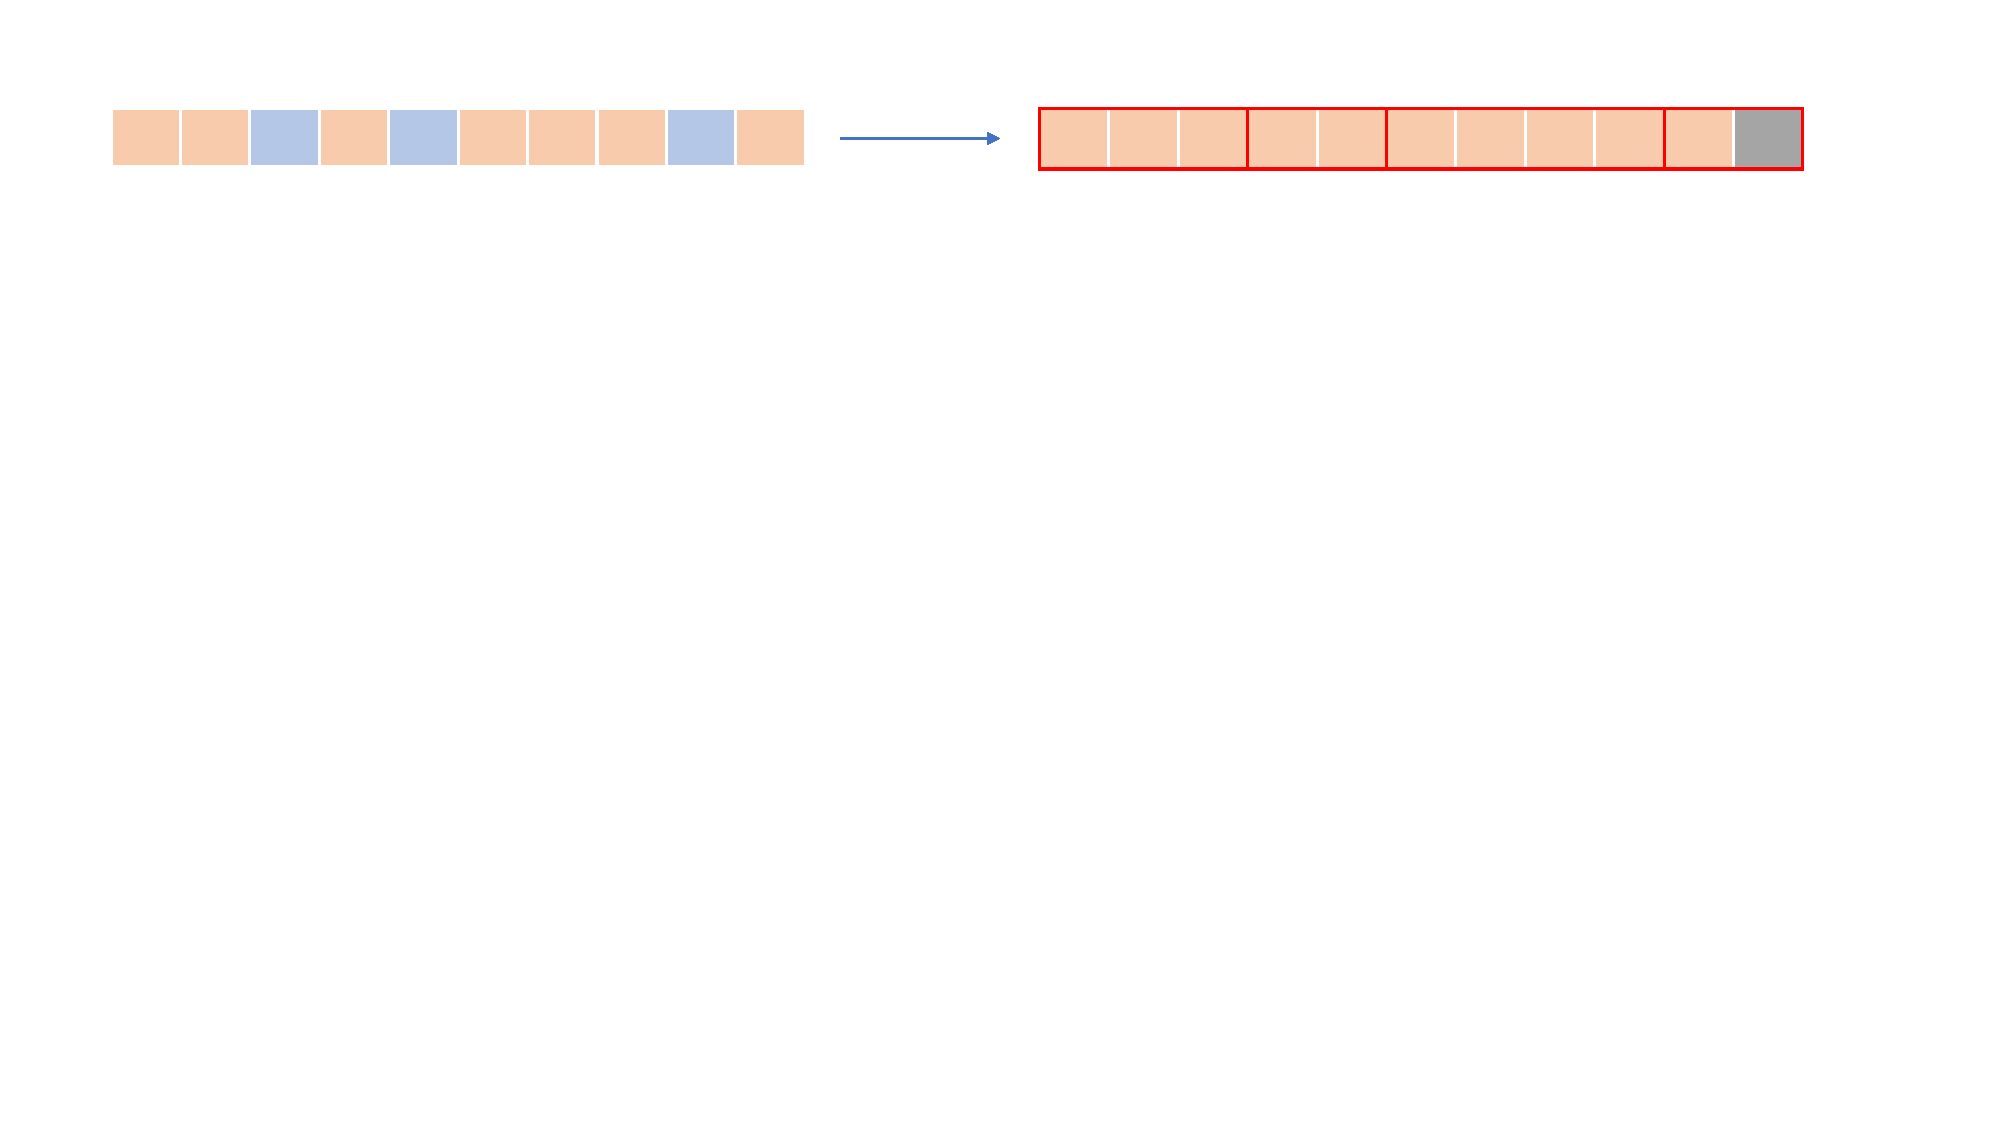
\includegraphics[width = 0.8\textwidth]{./images/dummy_seat.pdf}
      \caption{Problem Conversion with One Seat as Social Distancing}
  \end{figure}
  \end{frame}

  \begin{frame}{Basic Concepts}
    \begin{itemize}
      \item Pattern: $\bm{h} = (h_1, \ldots, h_M)$, the seat planning for one row whose length is $L$.

      - The number of people accommodated: $|\bm{h}| = \sum_{i =1}^{M} i h_i = qM + \max\{r-\delta, 0\}$, where $q = \lfloor L/(M + \delta) \rfloor$, $r \equiv L \bmod (M + \delta)$.
      
      \item $\bm{h}$ is a largest pattern if $|\bm{h}| \geq |\bm{h}^{\prime}|$ for any feasible $\bm{h}^{\prime}$. 
      \item $\bm{h}$ is a full pattern if $\sum_{i=1}^{M} n_i h_i = L$.
      \item[-] {\color{green} Example}: 
      
      $\delta = 1$, $M =4$, $L = 21$; $n_1 = 2, n_2 = 3, n_3 = 4, n_4 = 5$,
      
      Largest patterns: $(0, 0, 0, 4), (0, 0, 4, 1), (0, 2, 0, 3)$.

      Largest may not be full: $(0, 0, 0, 4)$.

      Full may not be largest: $(1, 1, 4, 0)$.
    \end{itemize}
  \end{frame}